\documentclass[11pt]{article} % scrbook otro formato
\usepackage[utf8]{inputenc}
\usepackage[spanish,es-tabla,es-nodecimaldot]{babel}

% Paquetes

\usepackage{amsmath}
\usepackage{amsthm}
\usepackage{amsfonts}
\usepackage{amssymb}
\usepackage{makeidx}
\usepackage{graphicx}
\usepackage{lmodern}
%\usepackage{kpfonts}
\usepackage{fancyhdr}
\usepackage{geometry}
\usepackage{lastpage}
\usepackage{array} % Para fjar tamaño de columnas
\RequirePackage{siunitx}
\usepackage{extramarks} % Para poder usar firstleftmarks
\usepackage[version=4]{mhchem} % Para poder usar formulas de reacciones nucleares
\usepackage{xcolor}
%\usepackage{newtxtext, newtxmath} % Cambia la fuente (pero mola)

%##############################################################################
%######### Ponemos el decimal con . ###########################################
%##############################################################################

\sisetup{output-decimal-marker={.},
	% exponentes ------------------------
	%exponent-mode=threshold,
	%exponent-thresholds=-3:2, % non usar exponentes 10^{-2,-1, 0, 1}
	% redondear -------------------------
	% round-mode=figures, % cifras sig
	% round-mode=places, % cantos decimales
	round-mode=uncertainty, % cifras sig da incerteza (necesario usar erro)
	round-precision=2,
	uncertainty-mode = separate,
	print-unity-mantissa=false,
	% unidades --------------------------
	inter-unit-product = \ensuremath{{}\cdot{}}, % separacion entre unidades
	% per-mode=power-positive-first, % so furrula con metodo interpretado puro
	inline-per-mode=single-symbol,
	display-per-mode=fraction,
}

%##############################################################################
%######### Para codigo python #################################################
%##############################################################################

\definecolor{codegreen}{rgb}{0,0.6,0}
\definecolor{codegray}{rgb}{0.5,0.5,0.5}
\definecolor{codepurple}{rgb}{0.58,0,0.82}
\definecolor{backcolour}{rgb}{0.95,0.95,0.92}

\usepackage{listings}


%\lstdefinestyle{mystyle}{	backgroundcolor=\color{backcolour},   	commentstyle=\color{codegreen},	keywordstyle=\color{magenta},	numberstyle=\tiny\color{codegray},	stringstyle=\color{codepurple},	basicstyle=\ttfamily\footnotesize,	breakatwhitespace=false,         	breaklines=true,                 	captionpos=b,                    	keepspaces=true,                 	numbers=left,                    	numbersep=5pt,                  	showspaces=false,                	showstringspaces=false,	showtabs=false,                  	tabsize=2}

%\lstset{style=mystyle}
%\usepackage{background}     % Para manejar el fondo


%##############################################################################
%######### Tipo de fuente #################################################
%##############################################################################

%\usepackage{kpfonts}

%\usepackage{helvet} 
%\renewcommand{\familydefault}{\sfdefault}.

%\usepackage{fontspec} % Paquete necesario para seleccionar fuentes
%\setmainfont{Verdana} % Cambia la fuente principal a Verdana


%##############################################################################
%######### Geometría #################################################
%##############################################################################

\geometry{a4paper, total={152mm,237mm}, left=31mm, top=30mm}



%##############################################################################
%######### Formatos capítulo #################################################
%##############################################################################

%\usepackage[lmodern]{quotchap}
%\usepackage[Bjornstrup]{fncychap}

% Para el Bjornstrup
%\ChNumVar{\fontsize{76}{80}\usefont{OT1}{pzc}{m}{n}\selectfont}
%\ChTitleVar{\raggedright\Huge\sffamily\bfseries}


%##############################################################################
%######### Hiperreferenias #################################################
%##############################################################################


\usepackage[colorlinks=true,allcolors=blue]{hyperref} % Crea las


%##############################################################################
%######### Formato de pagina #################################################
%##############################################################################

%\renewcommand{\chaptermark}[1]{\markboth{\chaptername\ \thechapter.\ #1}{}}
\renewcommand{\sectionmark}[1]{\markright{\thesection.\ #1}}

\setlength{\headsep}{27pt} % Distancia entre la cabezera y el texto
\setlength{\footskip}{30pt} % Distancia entre el pie de pagina y el texto
\pagestyle{fancy}
\fancyhf{}
\fancyhead[LE]{\rightmark} % L,R,C-> left, right, center [LE,RO]
\fancyhead[RO]{\rightmark} % E,O -> even (par), odd (impar)
\fancyhead[LO,RE]{Daniel Vázquez Lago}
\fancyfoot[CE,CO]{\thepage}
\renewcommand{\headrulewidth}{1pt} % Cambiamos el grosor de la linea de arriba
\renewcommand{\footrulewidth}{0pt}



%##############################################################################
%#########  Modificar caption #################################################
%##############################################################################

\usepackage[font=small, justification=centering]{caption}  % Configura las captions



%##############################################################################
%######### Comandos propios #################################################
%##############################################################################

\newcommand{\parentesis}[1]{\left( #1  \right)} 
\newcommand{\parciales}[2]{\frac{\partial #1}{\partial #2}}
\newcommand{\pparciales}[2]{\parentesis{\parciales{#1}{#2}}}
\newcommand{\ccorchetes}[1]{\left[ #1  \right]}
\newcommand{\D}{\mathrm{d}}
\newcommand{\derivadas}[2]{\frac{\D #1}{\D #2}}

\newcommand{\tquad}{\quad \quad \quad}
\newcommand{\vnabla}{\vec{\nabla}}

\newcommand{\Ocal}{\mathcal{O}}
\newcommand{\Ncal}{\mathcal{N}}
\newcommand{\Hcal}{\mathcal{H}}

\newcommand{\logd}{\log_{10}}

\newcommand{\eV}{\text{eV}}
\newcommand{\cm}{\text{cm}}
\newcommand{\cmm}{\text{cm}^{-1}}
\newcommand{\fm}{\text{fm}}
\newcommand{\He}{\text{He}}
\newcommand{\p}{\text{p}}
\newcommand{\e}{\text{e}}
\newcommand{\cte}{\text{cte}}


% Comandos vectoriales

\newcommand{\an}{\mathbf{a}}
\newcommand{\bn}{\mathbf{b}}
\newcommand{\dn}{\mathbf{d}}
\newcommand{\jn}{\mathbf{j}}
\newcommand{\lnn}{\boldsymbol{\ell}}
\newcommand{\lnnn}{\boldsymbol{l}}
\newcommand{\kn}{\mathbf{k}}
\newcommand{\pn}{\mathbf{p}}
\newcommand{\qn}{\mathbf{q}}
\newcommand{\rn}{\mathbf{r}}
\newcommand{\sn}{\mathbf{s}}
\newcommand{\un}{\mathbf{u}}
\newcommand{\vn}{\mathbf{v}}
\newcommand{\xn}{\mathbf{x}}
\newcommand{\yn}{\mathbf{y}}
\newcommand{\qndot}{\dot{\qn}}

\newcommand{\unovec}{\vec{\mathbf{1}}}

\newcommand{\alphan}{\boldsymbol{\alpha}}
\newcommand{\sigman}{\boldsymbol{\sigma}}
\newcommand{\pin}{\boldsymbol{\pi}}


\newcommand{\An}{\mathbf{A}}
\newcommand{\Bn}{\mathbf{B}}
\newcommand{\En}{\mathbf{E}}
\newcommand{\Gn}{\mathbf{G}}
\newcommand{\Jn}{\mathbf{J}}
\newcommand{\Kn}{\mathbf{K}}
\newcommand{\Ln}{\mathbf{L}}
\newcommand{\Rn}{\mathbf{R}}
\newcommand{\Sn}{\mathbf{S}}
\newcommand{\Tn}{\mathbf{T}}
\newcommand{\In}{\mathbf{I}}

\newcommand{\hnn}{\hat{\mathbf{n}}}
\newcommand{\hnr}{\hat{\mathbf{r}}}
\newcommand{\hnz}{\hat{\mathbf{z}}}
\newcommand{\hnx}{\hat{\mathbf{x}}}
\newcommand{\hny}{\hat{\mathbf{y}}}
\newcommand{\hnu}{\hat{\mathbf{u}}}
\newcommand{\hnR}{\hat{\mathbf{R}}}
\newcommand{\hnv}{\hat{\mathbf{v}}}
\newcommand{\hnk}{\hat{\mathbf{k}}}
\newcommand{\hni}{\hat{\mathbf{i}}}
\newcommand{\hnj}{\hat{\mathbf{j}}}
\renewcommand{\hnk}{\hat{\mathbf{k}}}





%##############################################################################
%######### Teoremas/definiciones #################################################
%##############################################################################

%\theoremstyle{definition}
%\newtheorem{definition}{Definición}[chapter]
%\theoremstyle{theorem}
%\newtheorem{theorem}{Teorema}[chapter]




%##############################################################################
%######### Referncia para euccaiones y figuras ################################
%##############################################################################

%\numberwithin{equation}{section}
%\numberwithin{figure}{section}




%##############################################################################
%######### Documento #################################################
%##############################################################################


\author{Daniel Vazquez Lago}
\title{Simulación en física de materiales}


\begin{document}	
	
\maketitle
\newpage
\tableofcontents
\section{Objetivos}

El objetivo de esta segunda entrega de la asignatura es llegar a la posición de equilibrio de un sistema de 500 partículas, con una densidad $\rho=0.5$ y una energía $E=575$ (variables reducidas) a partir de una posición inicial fcc. Sin embargo para llegar al equilibrio primero debemos avanzar en el tiempo, es decir, hacer una simulación. En este proyecto veremos qué debemos implementar para poder calcular posiciones temporales sucesivas hasta la posición deseada. En el optativo 1 dos veremos si, realmente con los pasos logrados en este ejercicio se llega o no al equilibrio.

\section{Organización}

En esta sección mencionare como están organizados el proyecto. En primer lugar hay que decir que, por motivos de organización personal, he creado una carpeta llamada \textit{Datos} donde se almacenan todos los \texttt{.dat} de todos los proyectos. Sin embargo para que se guarden correctamente he supuesto que se ejecuta desde el proyecto, esto es, desde el \texttt{.exe} que se genera al construir el proyecto. De hacerlo de otro modo esto llevaría a un error. En segundo lugar, se puede ver que tal y como recomendó el profesor, hay una carpeta donde guardo todos los archivos \texttt{.f95} (llamada \textit{Programas fuente}) y otra donde esta el proyecto \texttt{.ftn95p}, para así poder reusarlos y que esté bien ordenado. Una breve descripción de los archivos:

\begin{itemize}
	\item \textbf{Mod\_01\_Def\_prec}: modulo usado para definir las precisiones doble precisión y entero, permitiéndo usar datos con más cifras decimales.
	\item \textbf{Mod\_02\_Variables\_comunes}: nos permite pasar las variables comunes entre las diferentes subrutinas y programas sin necesidad de definirlos en los propios programas.
	\item \textbf{Mod\_03\_Interface}: módulo que nos permite detectar errores a la hora de introducir datos en las subrutinas, así como detectarlos en las variables de salida de las mismas.
	\item \textbf{Sub\_Potlj:} subrutina en la cual introducimos las posiciones y el número de partículas como variables de entrada y nos devuelve las aceleraciones/fuerzas, así como la energía potencial del sistema y sus derivadas respecto al volumen (primera y segunda).
	\item \textbf{Sub\_Verlet:} subrutina la cual recibe una configuración inicial en el instante $t$ y devuelve la nueva configuración inicial en $t+\Delta t$ (para esto esta subrutina llama a \texttt{Sub\_Potlj}). Además también obtenemos con ella la energía potencial.
	\item \textbf{Pro\_Equilibracion:} programa principal. Su principal función es leer la configuración inicial (partiendo de la fcc o bien de alguna más estable, siempre que verifique $E=-575$), y mediante un lazo iterar el número de veces que se desee la subrtuina \texttt{Sub\_Verlet}, avanzando un tiempo total $k\Delta t$, donde $k$ es el número de pasos y $\Delta t$ el intervalo temporal entre cada uno. Además escribirá en el mismo archivo que se leyó la configuración final, así como en nuevos archivos de datos las energías cinética, potencial y total; así como las velocidades (entre otros datos), en pos de ver si realmente se ha equilibrado.
\end{itemize}


\section{Simulación}

En esta sección vamos a ver como se hace la simulación, esto es, como calculamos la posición, velocidad... en la configuración $t+\Delta t$ a partir de los datos en $t$ (o anteriores, esto es, $t  - \Delta t, \ t - 2 \Delta t$). Primero haremos la introducción teórica, para luego ver la implementación práctica.

\subsection{Introducción teórica}

Para conocer la posición de las partículas en el instante de $t + \Delta t$, si $\Delta t$ es suficientemente pequeña, podemos desarrollar la serie de Taylor de $\rn(t+\Delta t)$

\begin{eqnarray}
	\rn(t+\Delta t) = \rn (t) + \dot{\rn} (t) \Delta t + \frac{1}{2} \ddot{\rn} (t) (\Delta T)^2 + \frac{1}{6} \dddot{\rn} (t) (\Delta T)^3 + \ldots
\end{eqnarray}
Conocidos los valores de $\rn,\dot{\rn}$, $\ddot{\rn}...$ podremos calcular la nueva posición. Sin embargo esto nos lleva a dos preguntas ¿A qué nos referimos con $\Delta t$ suficientemente pequeña?¿Qué valor le asignamos a las variables $\dot{\rn}...$? La primera pregunta la responderemos más adelante, respondamos por ahora a la segunda. Para conocer los valores de los diferentes $\dot{\rn}$ debemos usar las ecuaciones canónicas de nuestro hamiltoniano  $\Hcal$, dado por la energía cinética y un potencial que solo depende de la posición:

\begin{eqnarray}
	\Hcal = \sum_{i=1} \frac{\pn_i^2}{2m} + \varphi (\rn_i)
\end{eqnarray}
donde $\varphi(\rn_i)$ viene dado por el \textit{potencial Lennard-Jones}. Si definimos la velocidad como $\pn=m\vn$ y la aceleración como $\ddot{\rn}_i = \an_i$, tenemos que:

\begin{eqnarray}
	\dot{\rn}_i = \parciales{\Hcal}{\pn_i} = \frac{\pn_i}{m} = \vn_i
\end{eqnarray}

\begin{eqnarray}
	\dot{\pn}_i = - \parciales{\Hcal}{\rn_i} \Rightarrow  m \ddot{\rn}_i = - \parciales{\varphi(\rn_i)}{\rn_i} \Rightarrow \an_i =  - \frac{1}{m} \parciales{\varphi(\rn_i)}{\rn_i}
\end{eqnarray}
Una vez tenemos esto es sencillo ver que:
\begin{eqnarray}
	\dot{\rn}_i = \vn_i \tquad \an_i = - \parciales{\varphi(\rn_i)}{\rn_i}
\end{eqnarray}
Y por tanto podemos comprobar que 
\begin{eqnarray}
	\rn(t+\Delta t) = \rn(t) + \vn(t) \Delta t + \frac{1}{2} \an (t) (\Delta T)^2
\end{eqnarray}
donde hemos despreciado los términos de orden $(\Delta T)^3$ y superiores. Conocido  $\rn(t+\Delta t)$ calcular $\an(t+\Delta t)$ es trivial, ya que 

\begin{eqnarray}
	\an (t+\Delta t) = - \parciales{\varphi (\rn_i)}{\rn_{i}(t+\Delta t)}
\end{eqnarray}
Para obtener el valor de la velocidad podríamos usar el resultado más intuitivo según lo dicho, que sería $\vn(t+\Delta t) = \vn_i (t) + \an_i (t) \Delta t$. Sin embargo este no es estable (la estabilidad está relacionada con el error acumulado en las últimas cifras de los números con los que trabaja el ordenador, ya que nosotros hablamos de números reales y el ordenador de números decimales finitos). Un promedio estable sería:

\begin{eqnarray}
	\vn(t+\Delta t) & = & \vn(t) + \frac{1}{2} \parentesis{\an(t+\Delta t)+ \an(t)} \\
\end{eqnarray}
Este es el denominado \textbf{algoritmo velocity Verlet}. Aunque existen mas algoritmos, nosotros usaremos este porque es el más sencillo de implementar y funciona bien, sobretodo a bajas energías, como la nuestra. Escribiendo las ecuaciones todas juntas vemos que

\begin{eqnarray*}
	\rn(t+\Delta t) & = & \rn(t) + \vn(t) \Delta t + \frac{1}{2} \an (t) (\Delta T)^2 \\
	\vn(t+\Delta t) & = & \vn(t) + \frac{1}{2} \parentesis{\an(t+\Delta t)+ \an(t)} \\
	\an(t+\Delta t) & = &  - \parciales{\varphi(\rn_i)}{\rn_i}
\end{eqnarray*}


\subsection{Resultados}

Una vez corremos la simulación ($k_{\text{pasos}}=5000$, $\Delta t=\num{1e-4}$), obtenemos los resultados de la energía que vemos en la figura \ref{Fig:01}. 

\begin{figure}[h!] \centering
	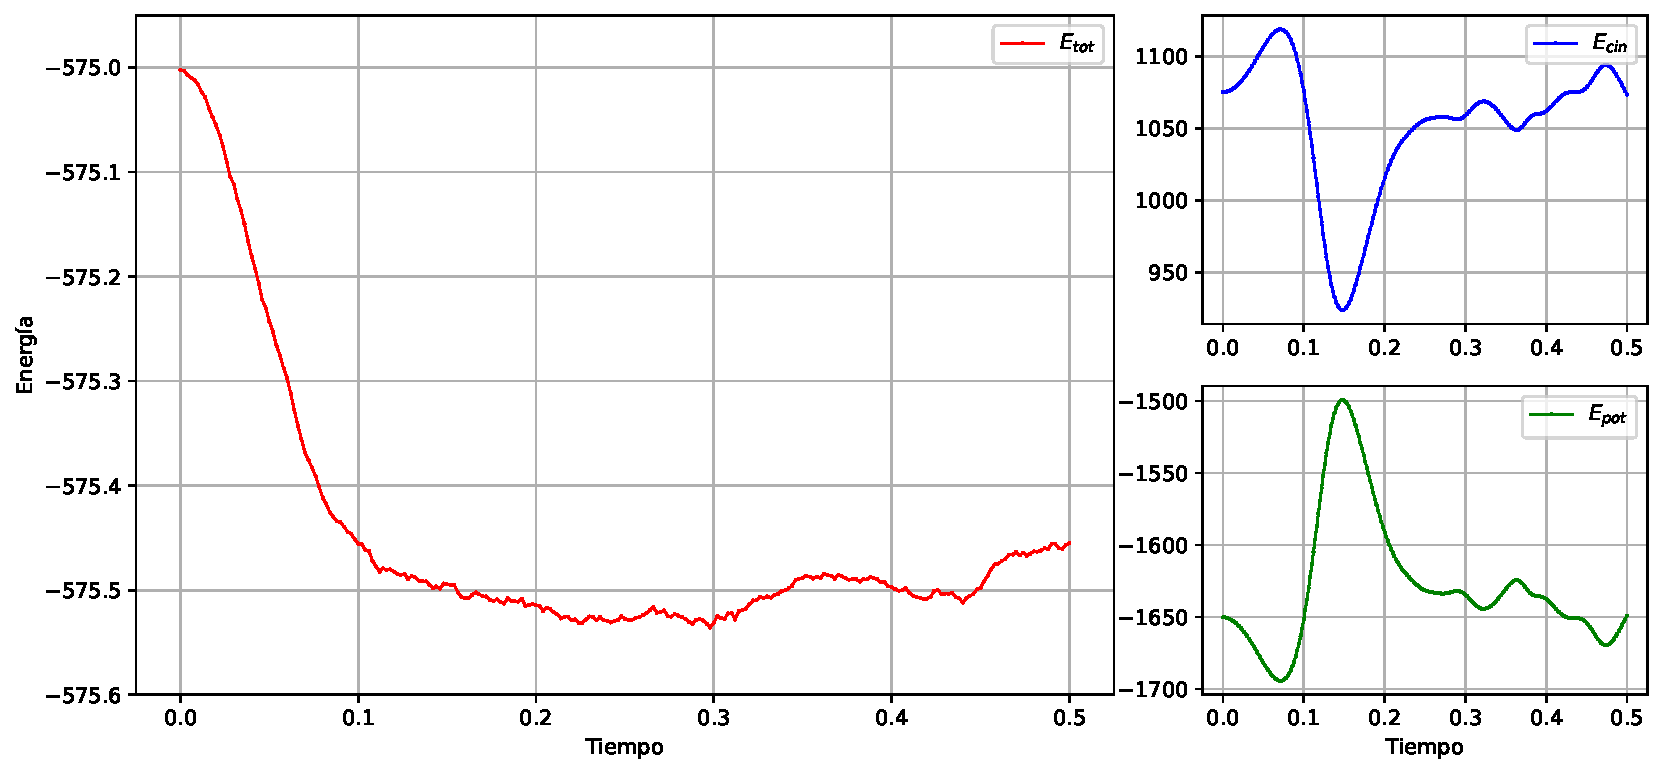
\includegraphics[width=0.62\textwidth]{../../Graficas/Et-equilibra.pdf}
	\caption{evolución de la energía total desde la configuración fcc y 5000 pasos.}
	\label{Fig:01}
\end{figure}	


Como podemos ver existe una caída de energía total hacia $-575.5$ sobre la cual, tras los 2000 pasos comienza a oscilar, es decir, se comienza a equilibrar en $-575.5$. La razón por la que sucede esta caída tan repetida es que la configuración inicial es muy simétrica, y por tanto está muy lejos de la equilibración, por lo que su evolución corresponderá a otro tipo de simulación. Esto no nos interesa, ya que nosotros queremos que el sistema este equilibrado en -575. Entonces lo que tenemos que hacer se subir la energía total usando el mismo algoritmo usado para en la colocación inicial para reescalar las velocidades (adecuándose a la energía cinética que necesitamos para que $E=575$) y asegurándonos que el momento total se mantenga cero, volvemos a hacer la simulación.


\begin{figure}[h!] \centering
	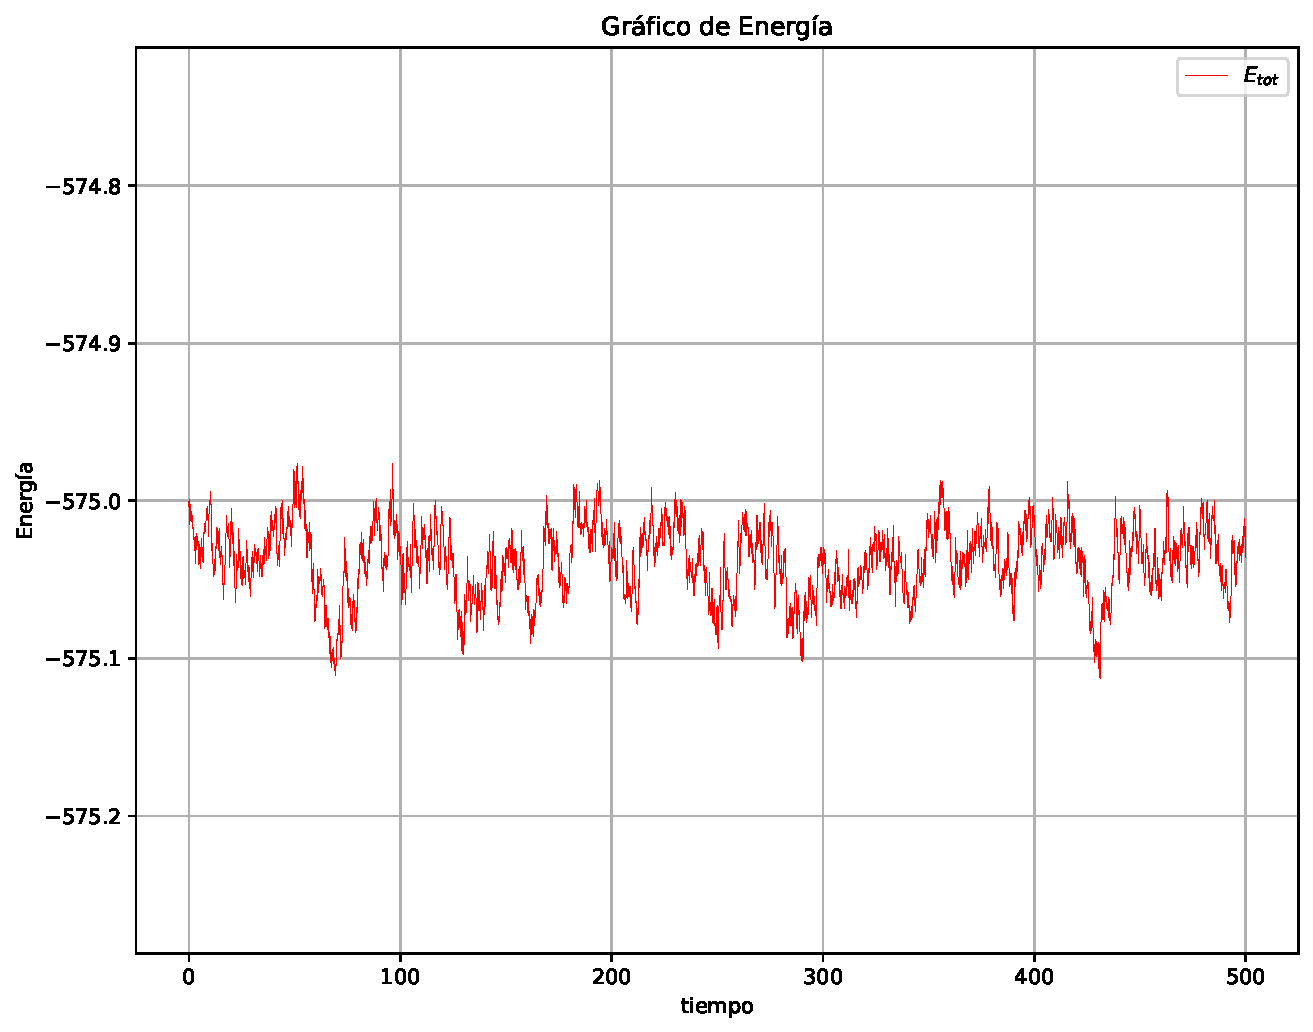
\includegraphics[width=0.63\textwidth]{../../Graficas/Et-equilibra-500K.pdf}
	\caption{evolución de la energía total 500000 pasos.}
	\label{Fig:04}
\end{figure}	

Como podemos ver, a diferencia de la anterior inicialización, en esta no habrá un salto de energía, ya que al haber dejado que ocurrieran 5000 pasos (aunque fuera en otra colectividad microcanónica), la configuración de las partículas ya no es simétrica, y por tanto estará mucho más cerca del equilibrio en la colectividad deseada, por lo que ahora podemos hacer un número mucho más elevado de pasos. Con $\num{5e5}$ serán suficientes. Ahora lo que resta sería usar los datos de las energías cinéticas, potenciales, totales, así como las velocidades de cada una de las 500 partículas en las 3 direcciones (entre otros) para ver si realmente hemos llegado al equilibrio. Esto, sin embargo, lo dejaremos para el optativo 1.

\section{Conclusiones}




\begin{figure}[h!] \centering
	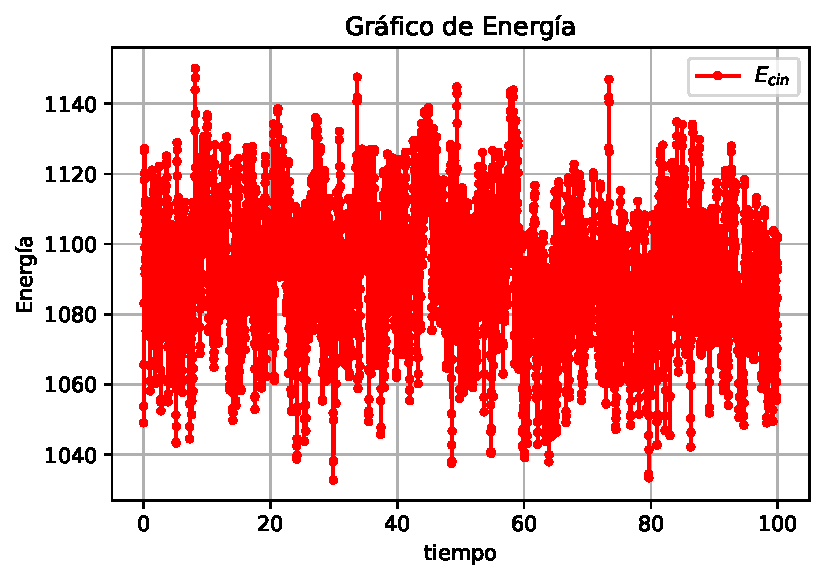
\includegraphics[width=0.9\textwidth]{../../Graficas/Ecin-equilibra.pdf}
	\caption{evolución de la energía cinética desde la configuración fcc y 5000 pasos.}
	\label{Fig:02}
\end{figure}	

\begin{figure}[h!] \centering
	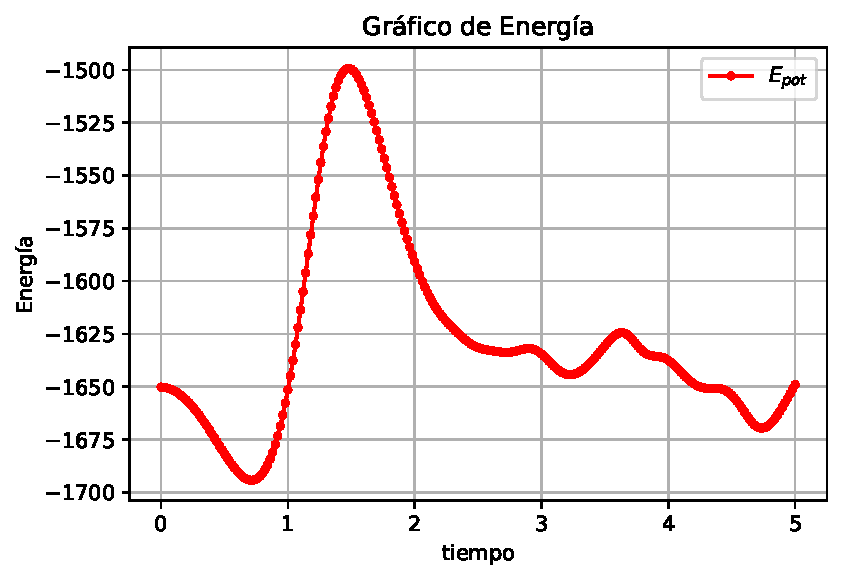
\includegraphics[width=0.9\textwidth]{../../Graficas/Epot-equilibra.pdf}
	\caption{evolución de la energía potencial desde la configuración fcc y 5000 pasos.}
	\label{Fig:03}
\end{figure}	

\begin{figure}[h!] \centering
	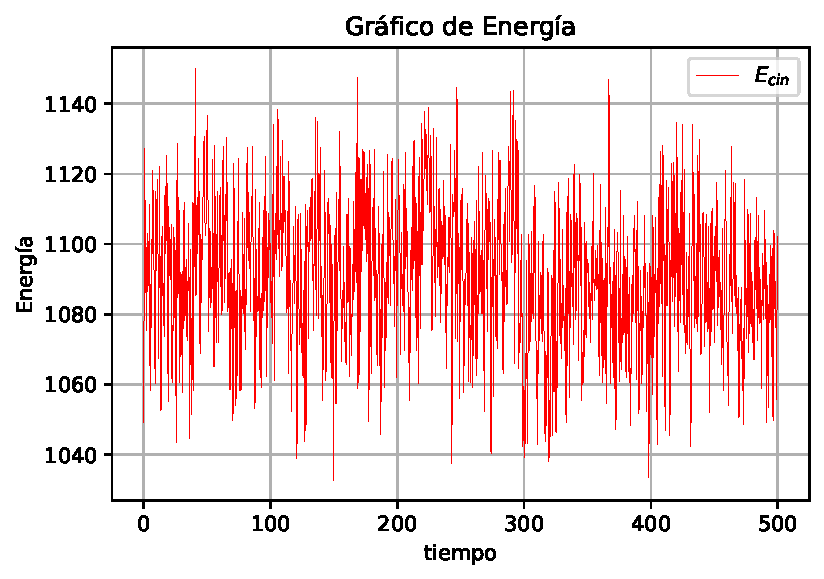
\includegraphics[width=0.9\textwidth]{../../Graficas/Ecin-equilibra-500K.pdf}
	\caption{evolución de la energía cinética 500000 pasos.}
	\label{Fig:05}
\end{figure}	

\begin{figure}[h!] \centering
	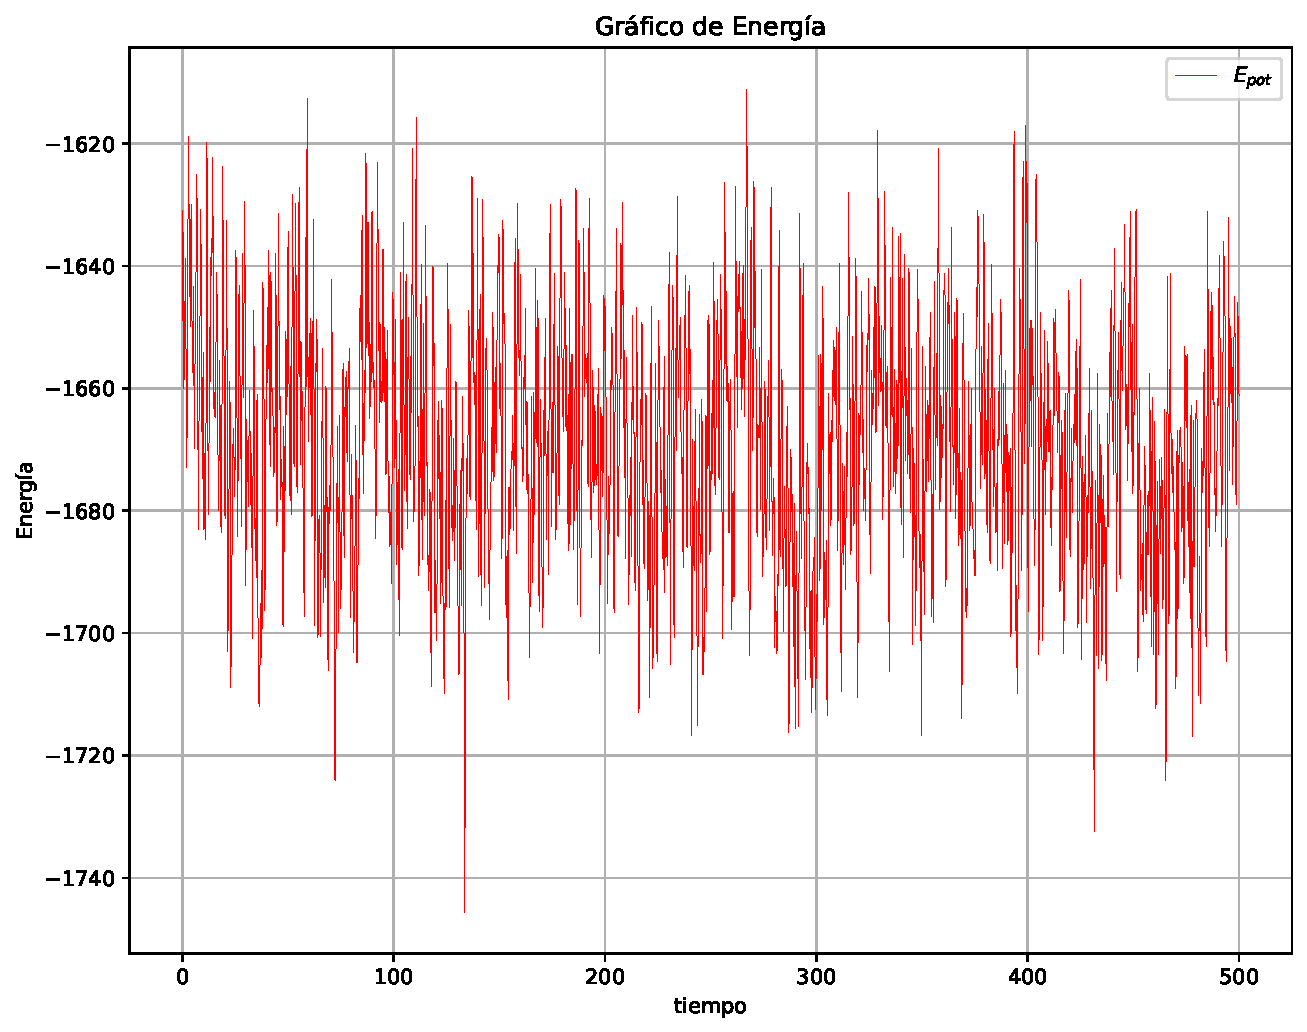
\includegraphics[width=0.9\textwidth]{../../Graficas/Epot-equilibra-500K.pdf}
	\caption{evolución de la energía potencial 500000 pasos.}
	\label{Fig:06}
\end{figure}	
\bibliography{Bibliografia.bib}
\bibliographystyle{unsrt}
	
\end{document}	
